\section{Simultaneous Localization and Mapping}
\label{slam}

In this section, we cover SLAM, and the different concepts related to SLAM such as Visual Odometry. We then explore the two different approaches to SLAM mentioned in the paper. We briefly cover filter based SLAM called MonoSLAM~\cite{davison2007monoslam} and a key-frame based SLAM called Parallel Tracking and Mapping (PTAM)~\cite{klein2007parallel}. A comprehensive analysis of filtering based SLAM is given in~\cite{strasdatavisual}. Simultaneous Localization and Mapping (SLAM) is a technique for estimating the motion of the robot and reconstructing the map/structure of the unknown environment. SLAM using only visual information only is specifically referred to as visual SLAM (vSLAM). The SLAM problem can be stated as follows:\\

\textbf{\emph{How can a body navigate in a previously unknown environment while constantly building and updating a map of its workspace using onboard sensors only?} ~\cite{chli2017}}\\

Mathematically, this can be expressed as~\cite{cyrillslam}

Input:\
\begin{equation}
Control\ input:\ u_{1:T} = {u_1, u_2, ...., u_T}
\end{equation}
\begin{equation}
Observations:\ z_{1:T} = {z_1, z_2, ...., z_T}
\end{equation}

Output:\
\begin{equation}
Map\ of\ Environment:\ m
\end{equation}
\begin{equation}
Path\ of\ robot:\ x_{0:T} = {x_0, x_1, ...., x_T}
\end{equation}

From the problem statement above, we notice that the robot has no a priori knowledge of the workspace or environment that it is in. This makes SLAM a very challenging problem in probabilistic robotics. This is also referred to as a chicken-egg problem in that we need to map the environment to get an accurate pose, but at the same time we also need an accurate pose to build a correct map. Therefore, it is an iterative process of estimating pose and building a map simultaneously. Accurate pose estimation is critical for many applications in computer vision, autonomous robotics and augmented reality. A survey of SLAM implementations is given in ~\cite{bresson2017simultaneous,cadena2016past,taketomi2017visual}. The basic modules for a vSLAM system are
\begin{itemize}
\item Initialization
\item Tracking
\item Mapping
\item Relocalization
\item Global Map optimization
\end{itemize}

According to~\cite{scaramuzza2011visual}, the relationship between vSLAM and VO can be represented as follows\\

$vSLAM = VO + global\ map\ optimization$\\


% For one-column wide figures use
\begin{figure}
% Use the relevant command to insert your figure file.
% For example, with the graphicx package use
  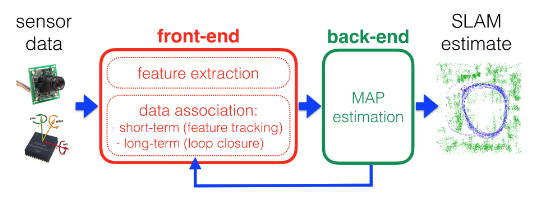
\includegraphics[width=\textwidth]{./figures/slam_model.png}
% figure caption is below the figure
\caption{SLAM architecture~\cite{cadena2016past}}
\label{fig:slammodel}       % Give a unique label
\end{figure}

From Fig~\ref{fig:slammodel} we see that a typical SLAM system consists of a front-end and a back-end. The front-end is responsible for feature extraction while the back-end is responsible for MAP estimation. Both the methods (MonoSLAM \& PTAM) are feature based implementations. 

\subsection{Visual Odometry}

Odometry is the technique of estimating the position of a robot over time using sensors such as cameras,  wheel encoders or any sensor measuring relative movement. Compared to SLAM which maintains a global consistent map, visual odometry (VO) maintains a local consistent map optimized over the last n frames. A generalized VO pipeline can be summarized as follows

% For one-column wide figures use
\begin{figure}[!htb]
% Use the relevant command to insert your figure file.
% For example, with the graphicx package use
  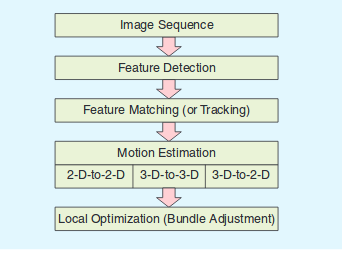
\includegraphics[width=\textwidth,height=5cm,keepaspectratio]{./figures/vo.png}
% figure caption is below the figure
\caption{Generalized Visual Odometry Pipeline~\cite{scaramuzza2011visual}}
\label{fig:vo}       % Give a unique label
\end{figure}

Different algorithms exist due to the different type of cameras available such as Stereo, Mono, RGB-D~\cite{scaramuzza2011visual,fraundorfer2012visual}. As we use a monocular setup in our research paper, we would be going through the visual odometry algorithm from 2D to 2D correspondences for a monocular sensor. The algorithm is summarized as follows~\cite{scaramuzza2011visual}.

\begin{algorithm}[H]
    \caption{Monocular Visual Odometry}
	\begin{algorithmic}[1]
		\STATE Capture a new image frame $I_k$
    	\STATE Extract and match features between frames $I_k$ and $I_{k-1}$
    	\STATE Compute the essential matrix $E$ from the matched feature points
    	\STATE Decompose $E$ into $R_k$ and $t_k$ to form $T_k$
    	\STATE Choose the correct $T_k$ matrix and scale $t_k$ accordingly from scale factor
    	\STATE Compute $C_k$ = $C_{k-1}*T_k$
    	\STATE Goto step 1.
	\end{algorithmic}
\end{algorithm}

Since we are using a monocular sensor, we always compare the image $I_k$ captured at time instant $k$ with the image $I_{k-1}$ capture at time instant $k-1$. In a stereo setup, we would compare images from the left and right part of the stereo. Once an image is captured, we compute the features for image $I_k$ and $I_{k-1}$. In the feature detection step, the image is searched for key-points called features  which are likely to be present in successive images. Features can be defined as image patterns that differ from its immediate neighborhood in terms of intensity, color and texture. There exist a variety of feature detectors in literature which vary in performance and properties. Some of the properties of feature detectors are rotation, scale and affine invariant, repeatability, localization accuracy, robustness and efficiency.  Heitanen et al. present a comparison of feature detectors and descriptors for object class matching in~\cite{hietanen2016comparison}. Once we detect features, we then need to compute a descriptor such that features detected in two images can be compared with each other. The easiest approach would be to form a patch of pixels and compare using a sum of squared distances (SSD) or normalized cross correlation (NCC) metric. Such descriptors are not invariant to any of the above mentioned properties and perform poorly in practical applications. One of the popular descriptors called SIFT~\cite{lowe2004distinctive} uses gradient orientations as its descriptors. This forms a 128-element descriptor that is invariant to most of the above mentioned properties such as rotation, scale and illumination which makes it widely applicable in practical real-time applications. For extracting features from two images there are two paths with one being to detect and match features independently in two frames and the other being to track features in subsequent frames an example of which is a KLT Tracker~\cite{tomasi1991detection}. There are various methods employed to match features accurately such a RANSAC which stands for Random Sample Consensus and is used to remove outliers among feature matches. Once we detect and match features in $I_k$ and $I_{k-1}$, we calculate the essential matrix $E$ which describes the geometric relationship between two images. We can use Nister’s five point algorithm~\cite{nister2004efficient} or Longuet-Higgins eight point algorithm~\cite{longuet1981computer} to get the essential matrix $E$. Once we get the essential matrix $E$, we decompose it to extract the rotation and translation parts. Four different solutions are obtained of which the correct pair can be found out by triangulation. The solutions are given as

\begin{equation}
	R = U(\pm W^T)V^T
\end{equation}
\begin{equation}	
	t = U(\pm W^T)SV^T
\end{equation}

where R is the rotation matrix and t is the translation vector. 

\subsection{MonoSLAM}

MonoSLAM was developed by Davison et al.~\cite{davison2003real,davison2007monoslam}. It uses EKF as an estimator. In EKFSLAM, the state \textbf{x} space is represented by the robot state $\hat{x_\nu}$ along with the position of the different landmarks $\hat{y_i}$ that the robot observes. The state vector along with the covariance matrix can be represented as follows

\begin{equation}
\hat{x} = 
\begin{pmatrix}
  \hat{x_\nu} \\
  \hat{y_1} \\
  \hat{y_2} \\
  : 	\\
 \end{pmatrix}
P = 
\begin{pmatrix}
  P_{xx} & P_{xy1} & P_{xy2} & \cdots \\
  P_{y1x} & P_{y1y1} & P_{y1y2} & \cdots \\
  P_{y2x} & P_{y2y1} & P_{y1y2} & \cdots \\
  : & :     &     :     & \cdots \\
 \end{pmatrix}
\end{equation}

The covariance matrix is used to represent the first order uncertainty. As the robot moves around, new features are added to the state vector. It is important to note that the robot initialization is done by using a known object. The prediction and correction steps are performed as mentioned in the EKF algorithm in section~\ref{ekf_section}. One of the problems with this method is that the state vector becomes large when the number of land marks or key-points tracked increases. This increases the computation time.

\subsection{Parallel Tracking and Mapping (PTAM)}
\label{ptamtheory}

PTAM is a SLAM system specifically designed to track a hand-held camera in a small AR workspace. For real-time operation, PTAM splits the tracking and mapping threads into two separate tasks running in parallel. The tracking thread robustly tracks hand-held motion and the mapping thread produces a 3D map of the features. Although developed specific to AR applications, the concept of running operations on multiple threads was incorporated into future SLAM algorithms. 

The map consists of a collection of key-points/features that are located in a world frame $W$. They are represented in the homogeneous form. The map also contains key-frames which a instances of the frames taken from the hand-held camera. Each point is stored with a source key-frame. Unlike earlier methods which process each and every frame, this method only processes frames when there is sufficient information. Thus incremental mapping is replaced with a more computationally expensive batch method called bundle adjustment. 

The tracking algorithm can be summarized as follows.

\begin{algorithm}
    \caption{PTAM - Tracking Algorithm}
    \begin{algorithmic}[1]
		\STATE A new frame is captured and a prior pose estimate is generated from motion model.
    	\STATE Map points are projected into the image based on prior pose. 
    	\STATE Small number of features (50) are searched in the image.
    	\STATE The camera pose is updated from the feature matches.
    	\STATE Large number of points is re-projected and searched in the image.
    	\STATE Final pose estimate is computed from all matched found. 
    	\STATE Goto step 1.
    \end{algorithmic}
\end{algorithm}

PTAM is initialized by a lateral offset movement of the hand-held camera. This can be assumed as a stereo image for starting the mapping. The initial map is constructed using the 5 point algorithm~\cite{nister2004efficient} with arbitrary scale. As the camera moves, the key-frames increase from an initial two. Here, we only add key-frames if the tracking quality is good and a minimum of twenty frames has passed from the last keyframe. Bundle adjustemnt is iteratively performed to adjust the map based on a cost function. The mapping algorithm can then be summarized as.

\begin{algorithm}
    \caption{PTAM - Mapping Algorithm}
	\begin{algorithmic}[1]
		\REQUIRE \mbox{Stereo Initialization}
		\IF {New Keyframe}
			\STATE Update key-frame
			\STATE Integrate key-frame
			\STATE Add new features
		\ELSIF {Locally Converged}
			\IF {Globally Converged}
				\STATE Update data association
			\ELSE
				\STATE Global bundle adjust
			\ENDIF
		\ELSE
			\STATE Locally bundle adjust
		\ENDIF
		\STATE Sleep 5ms
		\STATE Goto step 1.
	\end{algorithmic}
\end{algorithm}

Finally when compared with Filter based SLAM, PTAM can handle thousands of features by splitting the tracking and mapping onto different threads on the CPU. We see that SLAM algorithms built now-a-days have used this philosophy to great success. 

\subsection{Results}
\subsubsection{Simulated and Real Data}

In the paper, the Kalman filter was simulated offline with simulated data from the spline fitting section. The two inputs to the Kalman filter were the position from the vision sensor and acceleration from the IMU. Three different approaches were taken. The first method is same as Eq. 7, the second method only uses the Z-axis which gives the states as $[\overrightarrow{x}_z, \overrightarrow{\nu}_z, \overrightarrow{\alpha}_z, \lambda]$ and the third uses only the X and Y-axis. 

% For one-column wide figures use
\begin{figure}
% Use the relevant command to insert your figure file.
% For example, with the graphicx package use
  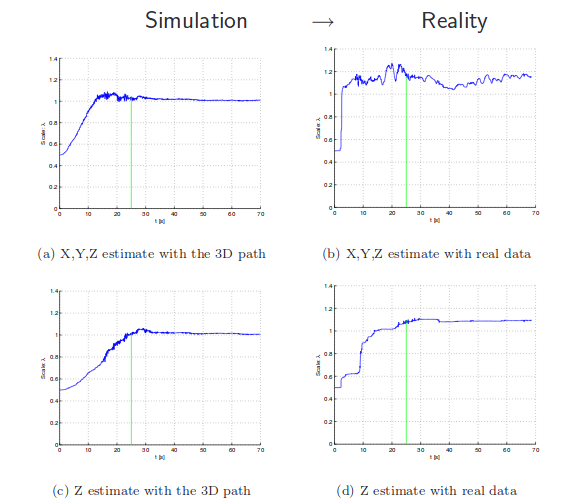
\includegraphics[width=\textwidth]{./figures/ekfTest.png}
% figure caption is below the figure
\caption{Offline simulation results with simulated and real data. Fewer directions (X,Y,Z) included in Kalman filter gives us a better estimate of $\lambda$.~\cite{nutzi2011fusion}}
\label{fig:ekf1}       % Give a unique label
\end{figure}

Figure~\ref{fig:ekf1} shows the scale estimation $\lambda(t)$ for a simulated 3D path on left and actual path on right. The standard deviation for the acceleration noise for simulation was chosen same as real data($\sigma_{SLAM} = 0.01, \sigma_{IMU} = 0.2 m/s^2$) with initial velocity and acceleration set to zero. Plots in Fig.~\ref{fig:ekf1}a and Fig.~\ref{fig:ekf1}c do not differ due to simulating the acceleration from the spline ideally in world frame. The estimate becomes more accurate when we use less number of directions (X,Y,Z).  Wrong measurements in acceleration influence $\lambda$ and make the scale estimation sensitive as seen in Fig.~\ref{fig:ekf1}b. Hence only using a single axis (Z-axis) gives us the best result. 


\subsubsection{Online Implementation}

For the online implementation, the third setup was incorporated into the PTAM code~\cite{ptamcode}. As mentioned in section~\ref{ptamtheory} PTAM employs two parallel threads called Tracker for tracking and MapMaker for mapping. Two additional threads for IMU and Kalman we added. The IMU thread provides the acceleration measurements. The Kalman thread starts with $\lambda$ calculated from integrating acceleration values, position from SLAM algorithm and acceleration and velocity set to 0. Values for covariance matrix \textbf{Q} is time-varied which provides control over the sensitivity of the Kalman filter. For our report we have not incorporated the online implementation and have reported results from the paper. 

% For one-column wide figures use
\begin{figure}
% Use the relevant command to insert your figure file.
% For example, with the graphicx package use
  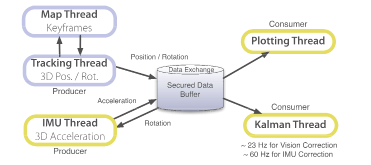
\includegraphics[width=\textwidth]{./figures/onlineEKF.png}
% figure caption is below the figure
\caption{Online implementation with PTAM work flow.Blue color boxes are original PTAM threads. Yellow boxes are added threads for scale estimation $\lambda$.~\cite{nutzi2011fusion}}
\label{fig:ekf2}       % Give a unique label
\end{figure}
